\documentclass[parskip=half, a4paper, DIV=14]{scrartcl}

\usepackage[ngerman,english]{babel}
\usepackage{helvet}
\usepackage{graphicx}
\usepackage{enumitem}

%http://de.wikibooks.org/wiki/LaTeX-W%C3%B6rterbuch:_fontfamily
\renewcommand{\familydefault}{\sfdefault}
\fontfamily{phv}\selectfont

\begin{document}

\title{Database System Project (SS 2015)}
\subtitle{MyMeal -- Documentation}
\author{Saulo Ribeiro de Andrade -- 7120309033\\
		Alexander Goscinski -- 7120309027\\
		Christan Würthner -- c.wuerthner@me.com}
\date{\today}
\maketitle

\tableofcontents
\newpage


\section{Database}
%Used database framework: MySQL ??% TODO version
In this chapter we introduce our database structure and explain design decisions as well as the meaning of every column.

For the database of our MyFood webpage service we created the following ER model.
\begin{figure}[h!]
	\centering
		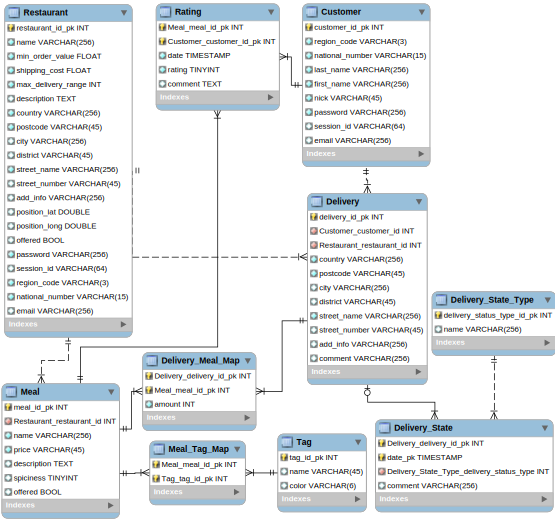
\includegraphics[scale=0.5]{er_model.png}
	\caption{ER model of our database.}
\end{figure}

We will now explain every column for every table.

	\subsection{Restaurant}
	The restaurant table represents the data of restaurant in real world.

	\setdescription{itemsep=5pt,parsep=0pt,leftmargin=0.5cm, style=sameline}
	\begin{description}
		\item[restaurant\_id\_pk: INT] This an automaticly generated surrogate key.
		\item[name: VARCHAR(256)] The name of the restaurant.
		\item[min\_order\_value: FLOAT] This value describes the minimum amount of value of a delivery so that a customer can submit a delivery.
	\end{description}

	\subsection{Delivery\_State}
	delivery state should be uniquely identified with the Delivery and time

\subsection{Dish}
We use the same

\subsection{Restaurant}
Text

\section{Server}
Text
\section{Front end}
Text


\end{document}

